\documentclass[aspectratio=169]{beamer}
\usepackage[utf8]{inputenc}
\usepackage[T1]{fontenc}
\usepackage{amsmath, amssymb}
\usepackage{booktabs}
\usepackage[table]{xcolor}
\usepackage{tikz}
\usepackage{background}
\usepackage{graphicx}
\usepackage{tikz-network}

% Configuración del tema
\usetheme{default}
\setbeamertemplate{navigation symbols}{}
\setbeamertemplate{headline}{}
\setbeamertemplate{footline}{}

% Paleta de colores azules profesionales
\definecolor{primaryblue}{RGB}{5, 35, 75}
\definecolor{secondaryblue}{RGB}{30, 90, 150}
\definecolor{accentblue}{RGB}{70, 160, 220}
\definecolor{lightblue}{RGB}{180, 210, 240}
\definecolor{textwhite}{RGB}{250, 250, 255}
\definecolor{darktext}{RGB}{20, 40, 70}

% Configuración de colores del tema
\setbeamercolor{frametitle}{fg=primaryblue}
\setbeamercolor{framesubtitle}{fg=secondaryblue}
\setbeamercolor{block title}{fg=white, bg=primaryblue}
\setbeamercolor{block body}{fg=darktext, bg=lightblue!20}
\setbeamercolor{alerted text}{fg=accentblue}

% Fuente más profesional
\usefonttheme{professionalfonts}

% Crear la red compleja como marca de agua
\newcommand{\networkwatermark}{%
	
\begin{tikzpicture}[remember picture, overlay, opacity=0.08]
		% Definir nodos de la red
		\coordinate (n1) at (current page.center);
		\coordinate (n2) at ([xshift=-3cm, yshift=2cm]current page.center);
		\coordinate (n3) at ([xshift=3cm, yshift=2.5cm]current page.center);
		\coordinate (n4) at ([xshift=-4cm, yshift=-2cm]current page.center);
		\coordinate (n5) at ([xshift=4cm, yshift=-1.5cm]current page.center);
		\coordinate (n6) at ([xshift=0cm, yshift=3.5cm]current page.center);
		\coordinate (n7) at ([xshift=-2cm, yshift=-3.5cm]current page.center);
		\coordinate (n8) at ([xshift=2.5cm, yshift=-3cm]current page.center);
		\coordinate (n9) at ([xshift=-5cm, yshift=1cm]current page.center);
		\coordinate (n10) at ([xshift=5cm, yshift=0.5cm]current page.center);
		\coordinate (n11) at ([xshift=-1.5cm, yshift=0cm]current page.center);
		\coordinate (n12) at ([xshift=1.5cm, yshift=-0.5cm]current page.center);
		
		% Conexiones de la red (aristas)
		\draw[secondaryblue, thick] (n1) -- (n2);
		\draw[secondaryblue, thick] (n1) -- (n3);
		\draw[secondaryblue, thick] (n1) -- (n4);
		\draw[secondaryblue, thick] (n1) -- (n5);
		\draw[secondaryblue, thick] (n1) -- (n6);
		\draw[secondaryblue, thick] (n1) -- (n7);
		\draw[secondaryblue, thick] (n1) -- (n8);
		\draw[secondaryblue, thick] (n1) -- (n11);
		\draw[secondaryblue, thick] (n1) -- (n12);
		
		\draw[accentblue, thick] (n2) -- (n6);
		\draw[accentblue, thick] (n2) -- (n9);
		\draw[accentblue, thick] (n2) -- (n11);
		\draw[accentblue, thick] (n3) -- (n6);
		\draw[accentblue, thick] (n3) -- (n10);
		\draw[accentblue, thick] (n3) -- (n12);
		\draw[accentblue, thick] (n4) -- (n7);
		\draw[accentblue, thick] (n4) -- (n9);
		\draw[accentblue, thick] (n4) -- (n11);
		\draw[accentblue, thick] (n5) -- (n8);
		\draw[accentblue, thick] (n5) -- (n10);
		\draw[accentblue, thick] (n5) -- (n12);
		\draw[accentblue, thick] (n7) -- (n11);
		\draw[accentblue, thick] (n8) -- (n12);
		\draw[accentblue, thick] (n9) -- (n11);
		\draw[accentblue, thick] (n10) -- (n12);
		\draw[accentblue, thick] (n11) -- (n12);
		
		% Nodos de la red
		\foreach \n in {n1,n2,n3,n4,n5,n6,n7,n8,n9,n10,n11,n12} {
			\fill[primaryblue] (\n) circle (0.15cm);
			\draw[accentblue, thin] (\n) circle (0.25cm);
		}
		
		% Conexiones adicionales para mayor complejidad
		\draw[secondaryblue, thin, dashed] (n6) -- (n9);
		\draw[secondaryblue, thin, dashed] (n6) -- (n10);
		\draw[secondaryblue, thin, dashed] (n7) -- (n9);
		\draw[secondaryblue, thin, dashed] (n8) -- (n10);
	\end{tikzpicture}%
}


% ---------------------------------------------------------
% MARCA DE AGUA: RED COMPLEJA LIBRE DE ESCALA
% ---------------------------------------------------------
\newcommand{\scalefreewatermark}{%
	
\begin{tikzpicture}[remember picture, overlay, opacity=0.05]
		% HUBS (nodos de alto grado - típicos de redes scale-free)
		\coordinate (H1) at ([shift={(4.5cm,2.2cm)}]current page.center);
		\coordinate (H2) at ([shift={(-3.8cm,-1.4cm)}]current page.center);
		\coordinate (H3) at ([shift={(1.8cm,-3.2cm)}]current page.center);
		\coordinate (H4) at ([shift={(-2.2cm,3.5cm)}]current page.center);
		
		% PERIFÉRICOS (20 nodos de bajo grado)
		\coordinate (P1)  at ([shift={(7cm,4cm)}]current page.center);
		\coordinate (P2)  at ([shift={(6cm,1.2cm)}]current page.center);
		\coordinate (P3)  at ([shift={(7.5cm,-1.5cm)}]current page.center);
		\coordinate (P4)  at ([shift={(3.5cm,5cm)}]current page.center);
		\coordinate (P5)  at ([shift={(2.8cm,-4.8cm)}]current page.center);
		\coordinate (P6)  at ([shift={(-5.5cm,4.2cm)}]current page.center);
		\coordinate (P7)  at ([shift={(-6.5cm,0.8cm)}]current page.center);
		\coordinate (P8)  at ([shift={(-4.8cm,-4.2cm)}]current page.center);
		\coordinate (P9)  at ([shift={(-0.8cm,5.2cm)}]current page.center);
		\coordinate (P10) at ([shift={(0.2cm,-5.2cm)}]current page.center);
		\coordinate (P11) at ([shift={(8.5cm,2.5cm)}]current page.center);
		\coordinate (P12) at ([shift={(-7.5cm,2.8cm)}]current page.center);
		\coordinate (P13) at ([shift={(4.5cm,-5.8cm)}]current page.center);
		\coordinate (P14) at ([shift={(-5.8cm,-2.8cm)}]current page.center);
		\coordinate (P15) at ([shift={(1.2cm,3.8cm)}]current page.center);
		\coordinate (P16) at ([shift={(-2.5cm,-3.8cm)}]current page.center);
		\coordinate (P17) at ([shift={(7cm,-2.8cm)}]current page.center);
		\coordinate (P18) at ([shift={(-7cm,-0.8cm)}]current page.center);
		\coordinate (P19) at ([shift={(4cm,4.8cm)}]current page.center);
		\coordinate (P20) at ([shift={(-4.5cm,5.8cm)}]current page.center);
		
		% Conexiones HUB → PERIFÉRICO (distribución de ley de potencia)
		\draw[accentblue, very thin] (H1) -- (P1) -- (P2) -- (P3) -- (P11) -- (H1);
		\draw[accentblue, very thin] (H1) -- (P4) -- (P19) -- (H1);
		\draw[accentblue, very thin] (H1) -- (P17) -- (H1);
		
		\draw[accentblue, very thin] (H2) -- (P6) -- (P7) -- (P12) -- (P18) -- (H2);
		\draw[accentblue, very thin] (H2) -- (P14) -- (P8) -- (H2);
		
		\draw[accentblue, very thin] (H3) -- (P5) -- (P13) -- (P16) -- (H3);
		\draw[accentblue, very thin] (H3) -- (P10) -- (P17) -- (H3);
		\draw[accentblue, very thin] (H3) -- (P15) -- (H3);
		
		\draw[accentblue, very thin] (H4) -- (P9) -- (P20) -- (P6) -- (H4);
		\draw[accentblue, very thin] (H4) -- (P7) -- (P12) -- (H4);
		\draw[accentblue, very thin] (H4) -- (P15) -- (P19) -- (H4);
		
		% Conexiones periférico-periférico (esparsas, para realismo topológico)
		\draw[secondaryblue, thin, dashed, opacity=0.6] (P1) -- (P11);
		\draw[secondaryblue, thin, dashed, opacity=0.6] (P4) -- (P9);
		\draw[secondaryblue, thin, dashed, opacity=0.6] (P5) -- (P13);
		\draw[secondaryblue, thin, dashed, opacity=0.6] (P8) -- (P14);
		
		% Dibujar nodos
		\foreach \h in {H1,H2,H3,H4} {
			\fill[accentblue, opacity=0.9] (\h) circle (4pt);
			\draw[accentblue, thick, opacity=0.5] (\h) circle (8pt);
		}
		\foreach \p in {P1,P2,P3,P4,P5,P6,P7,P8,P9,P10,P11,P12,P13,P14,P15,P16,P17,P18,P19,P20} {
			\fill[secondaryblue, opacity=0.5] (\p) circle (2.5pt);
		}
	\end{tikzpicture}%
}

% Aplicar la marca de agua a TODAS las diapositivas automáticamente
\setbeamertemplate{background canvas}{\scalefreewatermark}
% Estilo para bloques
\setbeamertemplate{blocks}[rounded][shadow=false]

\begin{document}
	
	% Diapositiva de título
	\begin{frame}[plain]
		\begin{tikzpicture}[remember picture, overlay]
			% Fondo gradiente azul
			\shade[top color=primaryblue, bottom color=secondaryblue, middle color=primaryblue!80] 
			(current page.south west) rectangle (current page.north east);
			
			% Red decorativa más visible en el centro
			\begin{scope}[opacity=0.3]
				\coordinate (c1) at ([xshift=-2cm, yshift=1cm]current page.center);
				\coordinate (c2) at ([xshift=2cm, yshift=1.5cm]current page.center);
				\coordinate (c3) at ([xshift=0cm, yshift=-2cm]current page.center);
				\coordinate (c4) at ([xshift=-3cm, yshift=-1cm]current page.center);
				\coordinate (c5) at ([xshift=3cm, yshift=-0.5cm]current page.center);
				
				\draw[accentblue, thick] (c1) -- (c2) -- (c3) -- (c4) -- (c5) -- (c1);
				\draw[accentblue, thick] (c1) -- (c3);
				\draw[accentblue, thick] (c2) -- (c4);
				\draw[accentblue, thick] (c2) -- (c5);
				
				\foreach \c in {c1,c2,c3,c4,c5} {
					\fill[lightblue] (\c) circle (0.2cm);
				}
			\end{scope}
			
			% Título
			\node[anchor=north, align=center, text width=0.9\paperwidth, text=textwhite, font=\bfseries\Large] 
			at ([yshift=-2cm]current page.north) 
			{Modelado Multiescala de la Red Metabólica del Cáncer de Mama};
			
			% Subtítulo
			\node[anchor=north, align=center, text width=0.8\paperwidth, text=lightblue, font=\normalsize] 
			at ([yshift=-4.5cm]current page.north) 
			{De la topología compleja a la dinámica espacial:\\ Redes PPI, Robustez y Patrones de Turing};
			
			% Autor
			\node[anchor=south, align=center, text width=0.8\paperwidth, text=textwhite, font=\small] 
			at ([yshift=2.5cm]current page.south) 
			{Alejandro Guerra González\\
				Asesor: Dr. Erik César Herrera Hernández\\
				Facultad de Ciencias Químicas, UASLP};
		\end{tikzpicture}
	\end{frame}
	
	% Índice
	\begin{frame}{Índice}
		\tableofcontents
	\end{frame}
	
	\section{Introducción y Justificación}
	
	\begin{frame}{El cáncer no es una célula aislada}
		\begin{columns}[T]
			\begin{column}{0.48\textwidth}
				\textbf{\color{primaryblue}Concepto Fundamental}
				\vspace{0.3cm}
				
				\begin{block}{Perspectiva Sistémica}
					\begin{itemize}
						\item El cáncer es una enfermedad de red
						\item Interacciones celulares complejas
						\item Microambiente tumoral dinámico
						\item Comunicación paracrina y autocrina
					\end{itemize}
				\end{block}
				
				\vspace{0.3cm}
				\begin{alertblock}{Importancia}
					Comprender la topología de red es esencial para identificar vulnerabilidades terapéuticas
				\end{alertblock}
			\end{column}
			
			\begin{column}{0.48\textwidth}
				\centering
				\only<1>{
					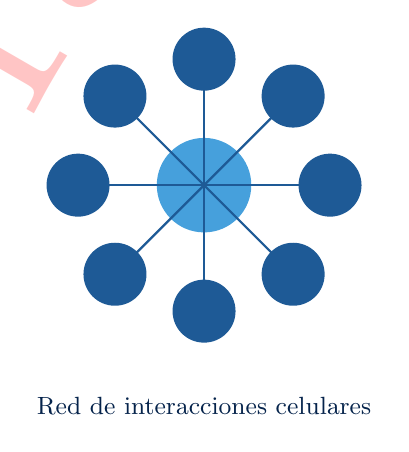
\begin{tikzpicture}[scale=0.8]
						% Representación visual de red celular
						\foreach \i in {1,...,8} {
							\node[circle, fill=secondaryblue, minimum size=0.8cm] at (360/8*\i:2cm) {};
						}
						\node[circle, fill=accentblue, minimum size=1.2cm] at (0,0) {};
						\foreach \i in {1,...,8} {
							\draw[secondaryblue, thick] (360/8*\i:2cm) -- (0,0);
						}
						\node[text=primaryblue, font=\small] at (0,-3.5) {Red de interacciones celulares};
					\end{tikzpicture}
				}
				\only<2->{
					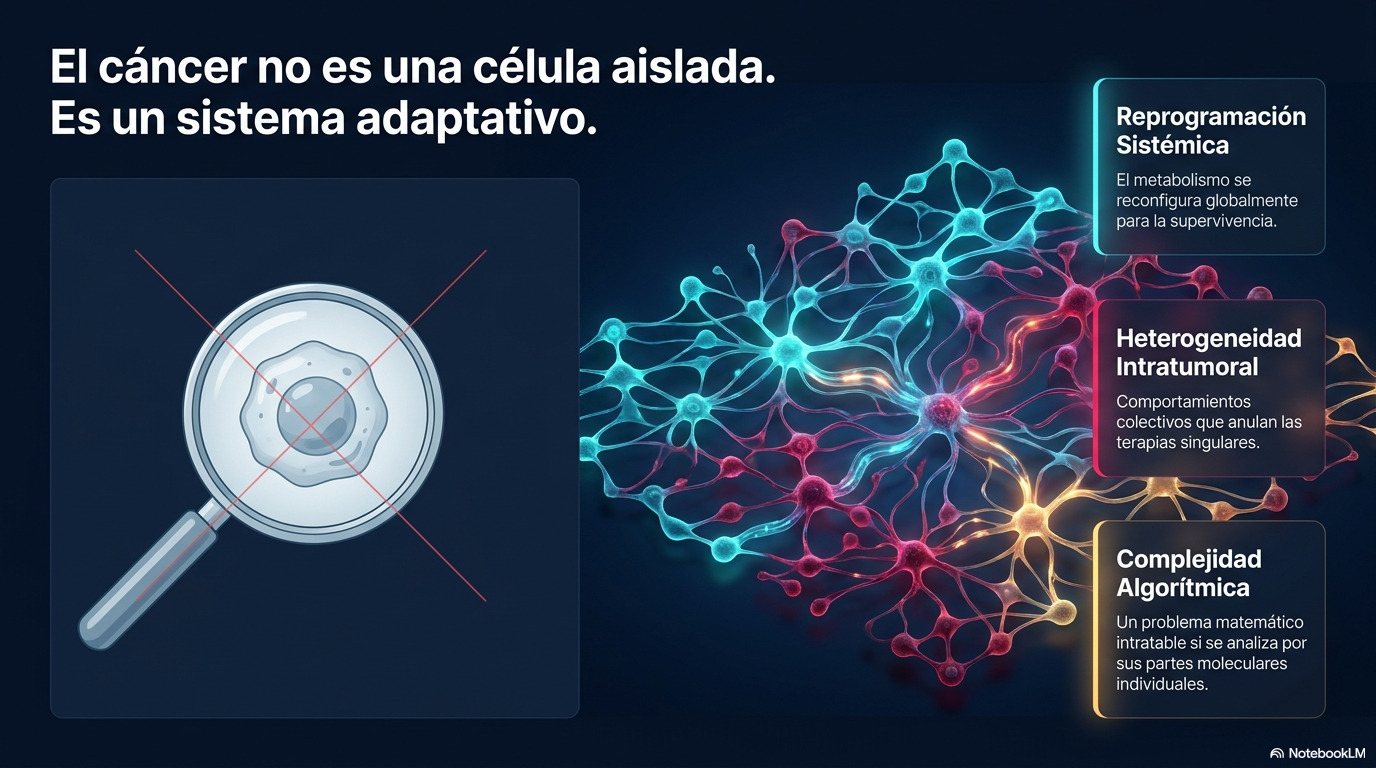
\includegraphics[width=\textwidth, height=0.7\textheight, keepaspectratio]{slide_1.jpeg}
				}
			\end{column}
		\end{columns}
	\end{frame}
	
	\begin{frame}{Topología Diferencial: El recableado genético}
		\begin{columns}[T]
			\begin{column}{0.48\textwidth}
				\begin{block}{\color{primaryblue}Célula Normal}
					\begin{itemize}
						\item Homeostasis estructural
						\item Distribución de grado equitativa
						\item Redes PPI operando bajo régimen basal y estable
						\item Control negativo funcional
					\end{itemize}
				\end{block}
				
				\vspace{0.3cm}
				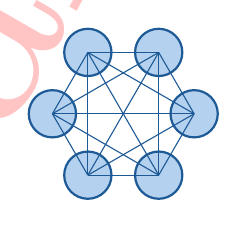
\begin{tikzpicture}[scale=0.6]
					\foreach \i in {1,...,6} {
						\node[circle, fill=lightblue, draw=secondaryblue, thick, minimum size=0.6cm] 
						at (360/6*\i:1.5cm) {};
					}
					\foreach \i in {1,...,6} {
						\foreach \j in {\i,...,6} {
							\draw[secondaryblue, thin] (360/6*\i:1.5cm) -- (360/6*\j:1.5cm);
						}
					}
				\end{tikzpicture}
			\end{column}
			
			\begin{column}{0.48\textwidth}
				\begin{alertblock}{\color{primaryblue}Célula Tumoral}
					\begin{itemize}
						\item Reprogramación topológica
						\item Análisis DCloc/DCglob revela módulos hiperconectados
						\item Cooperación de micro-ARN para plasticidad celular
						\item Pérdida de regulación
					\end{itemize}
				\end{alertblock}
				
				\vspace{0.3cm}
				\begin{alertblock}{Nodos de Vulnerabilidad}
					\textbf{FPR2 \& CXCR4:} Metástasis dirigida\\
					\textbf{GPR37:} Comunicación paracrina
				\end{alertblock}
			\end{column}
		\end{columns}
		
		\vspace{0.3cm}
		\begin{center}
			\footnotesize \textit{\color{secondaryblue}En una red de topología libre de escala, la metástasis es la ejecución de una red de comunicación celular}
		\end{center}
	\end{frame}
	
	\section{Conexión con Modelos Dinámicos}
	
	\begin{frame}{El problema de la traducción espaciotemporal}
		\begin{columns}[T]
			\begin{column}{0.48\textwidth}
				\begin{block}{\color{primaryblue}La Estructura}
					\centering
					\vspace{0.2cm}
					Grafos de Redes PPI Estáticas
					
					\vspace{0.3cm}
					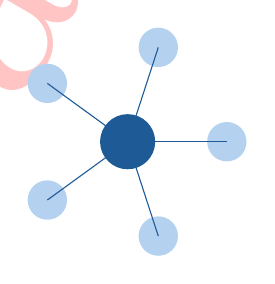
\begin{tikzpicture}[scale=0.7]
						\node[circle, fill=secondaryblue, minimum size=0.7cm] at (0,0) {};
						\foreach \i in {1,...,5} {
							\node[circle, fill=lightblue, minimum size=0.5cm] at (360/5*\i:1.8cm) {};
							\draw[secondaryblue] (0,0) -- (360/5*\i:1.8cm);
						}
					\end{tikzpicture}
				\end{block}
			\end{column}
			
			\begin{column}{0.04\textwidth}
				\centering
				\Huge \color{accentblue}$\rightarrow$
			\end{column}
			
			\begin{column}{0.48\textwidth}
				\begin{alertblock}{\color{primaryblue}El Fenotipo}
					\centering
					\vspace{0.2cm}
					Heterogeneidad y Metástasis en Espacio-Tiempo
					
					\vspace{0.3cm}
					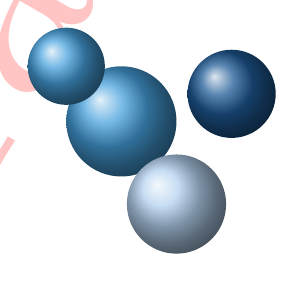
\begin{tikzpicture}[scale=0.7]
						\shade[ball color=accentblue] (0,0) circle (1cm);
						\shade[ball color=secondaryblue] (2,0.5) circle (0.8cm);
						\shade[ball color=lightblue] (1,-1.5) circle (0.9cm);
						\shade[ball color=accentblue] (-1,1) circle (0.7cm);
					\end{tikzpicture}
				\end{alertblock}
			\end{column}
		\end{columns}
		
		\vspace{0.4cm}
		\begin{quote}
			\centering
			\textit{\color{secondaryblue}¿Cómo se traduce la rigidez de una estructura matemática en el caos adaptable de un tumor biológico?}
		\end{quote}
		
		\vspace{0.3cm}
		\begin{center}
			\fbox{\parbox{0.6\textwidth}{\centering \textbf{\color{primaryblue}Solución: Modelado Dinámico Multiescala}}}
		\end{center}
	\end{frame}
	
	\section{Marco Teórico}
	
	\begin{frame}{Encontrando el orden oculto: Modularidad Metabólica}
		\begin{columns}[T]
			\begin{column}{0.32\textwidth}
				\centering
				\begin{block}{\color{primaryblue}Fase 1: Red Masiva}
					\vspace{0.2cm}
					\footnotesize
					Escala Mesoscópica\\
					\vspace{0.2cm}
					Descomposición matemática de la red masiva (KEGG/STRING)
				\end{block}
				
				\vspace{0.2cm}
				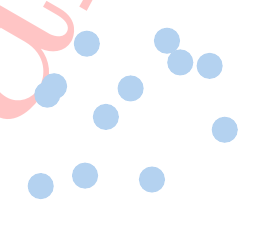
\begin{tikzpicture}[scale=0.5]
					\foreach \i in {1,...,12} {
						\node[circle, fill=lightblue, minimum size=0.3cm] at (rand*3, rand*3) {};
					}
				\end{tikzpicture}
			\end{column}
			
			\begin{column}{0.04\textwidth}
				\centering
				\Huge \color{accentblue}$\rightarrow$
			\end{column}
			
			\begin{column}{0.32\textwidth}
				\centering
				\begin{alertblock}{\color{primaryblue}Fase 2: Algoritmo de Louvain}
					\vspace{0.2cm}
					\footnotesize
					Detección Algorítmica\\
					\vspace{0.2cm}
					Comunidades altamente interconectadas
				\end{alertblock}
				
				\vspace{0.2cm}
				
\begin{tikzpicture}[scale=0.5]
					\foreach \i in {1,...,4} {
						\node[circle, fill=secondaryblue, minimum size=0.4cm] at (\i*0.8, 0) {};
					}
					\foreach \i in {1,...,4} {
						\node[circle, fill=accentblue, minimum size=0.4cm] at (\i*0.8, -1) {};
					}
				\end{tikzpicture}
			\end{column}
			
			\begin{column}{0.04\textwidth}
				\centering
				\Huge \color{accentblue}$\rightarrow$
			\end{column}
			
			\begin{column}{0.28\textwidth}
				\centering
				\begin{block}{\color{primaryblue}Fase 3: Comunidades Funcionales}
					\vspace{0.2cm}
					\footnotesize
					Coherencia Funcional\\
					\vspace{0.2cm}
					Módulos metabólicos vivos (ej. Glucólisis)
				\end{block}
				
				\vspace{0.2cm}
				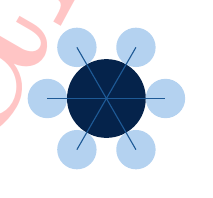
\begin{tikzpicture}[scale=0.5]
					\node[circle, fill=primaryblue, minimum size=1cm] at (0,0) {};
					\foreach \i in {1,...,6} {
						\node[circle, fill=lightblue, minimum size=0.5cm] at (360/6*\i:1.5cm) {};
						\draw[secondaryblue] (0,0) -- (360/6*\i:1.5cm);
					}
				\end{tikzpicture}
			\end{column}
		\end{columns}
	\end{frame}
	
	\begin{frame}{De la red a la ecuación: Reducción Dinámica}
		\begin{columns}[T]
			\begin{column}{0.48\textwidth}
				\begin{block}{\color{primaryblue}Ecuación Fundamental}
					\begin{equation*}
						\dot{x}_i = f(x_i) + \sum_{j} A_{ij} \, g(x_j, x_i)
					\end{equation*}
				\end{block}
				
				\vspace{0.3cm}
				\textbf{Componentes:}
				\begin{itemize}
					\item Actividad dinámica de la comunidad
					\item Dinámica interna del nodo
					\item Matriz de adyacencia (huella topológica)
				\end{itemize}
			\end{column}
			
			\begin{column}{0.48\textwidth}
				\begin{block}{\color{primaryblue}Separación de Escalas}
					\begin{itemize}
						\item Renormalización temporal
						\item Reducción de dimensionalidad
						\item Preservación de propiedades topológicas
					\end{itemize}
				\end{block}
				
				\vspace{0.3cm}
				\begin{columns}
					\begin{column}{0.48\textwidth}
						\begin{block}{Atractor Estable}
							\footnotesize Homeostasis controlada
						\end{block}
					\end{column}
					\begin{column}{0.48\textwidth}
						\begin{alertblock}{Régimen Caótico}
							\footnotesize Transición a malignidad
						\end{alertblock}
					\end{column}
				\end{columns}
			\end{column}
		\end{columns}
		
		\vspace{0.2cm}
		\begin{center}
			\footnotesize \textit{\color{secondaryblue}El sistema de EDO reducido permite evaluar sensibilidad y predecir puntos de bifurcación}
		\end{center}
	\end{frame}
	
	\begin{frame}{La paradoja de la supervivencia tumoral}
		\begin{columns}[T]
			\begin{column}{0.48\textwidth}
				\begin{block}{\color{primaryblue}1. Robustez Estructural (El Escudo)}
					\begin{itemize}
						\item Topología libre de escala
						\item La red sobrevive a perturbaciones aleatorias
						\item Resistencia a terapias estándar
						\item Redundancia funcional
					\end{itemize}
				\end{block}
				
				\vspace{0.3cm}
				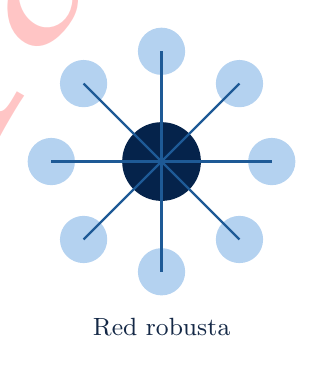
\begin{tikzpicture}[scale=0.7]
					\node[circle, fill=primaryblue, minimum size=1cm] at (0,0) {};
					\foreach \i in {1,...,8} {
						\node[circle, fill=lightblue, minimum size=0.6cm] at (360/8*\i:2cm) {};
						\draw[secondaryblue, thick] (0,0) -- (360/8*\i:2cm);
					}
					\node[text=darktext, font=\small] at (0,-3) {Red robusta};
				\end{tikzpicture}
			\end{column}
			
			\begin{column}{0.48\textwidth}
				\begin{alertblock}{\color{primaryblue}2. Inestabilidad Dinámica (El Motor)}
					\begin{itemize}
						\item Alta sensibilidad paramétrica
						\item Propensión a nuevos fenotipos (plasticidad)
						\item Respuesta rápida al estrés
						\item Adaptabilidad metabólica
					\end{itemize}
				\end{alertblock}
				
				\vspace{0.3cm}
				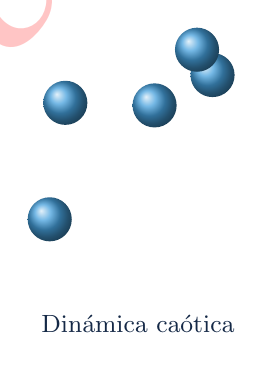
\begin{tikzpicture}[scale=0.7]
					\foreach \i in {1,...,5} {
						\shade[ball color=accentblue] (rand*2.5, rand*2.5) circle (0.4cm);
					}
					\node[text=darktext, font=\small] at (0,-3) {Dinámica caótica};
				\end{tikzpicture}
			\end{column}
		\end{columns}
		
		\vspace{0.4cm}
		\begin{center}
			\Large \textbf{\color{primaryblue}Robustez Estructural $\neq$ Estabilidad Dinámica}
		\end{center}
	\end{frame}
	
	\begin{frame}{Integrando el espacio: Sistemas de Reacción-Difusión}
		\begin{columns}[T]
			\begin{column}{0.48\textwidth}
				\begin{block}{\color{primaryblue}Ecuación de Reacción-Difusión}
					\begin{equation*}
						\frac{\partial x_i}{\partial t} = f(x_i) + D_i \nabla^2 x_i + \sum_{j} A_{ij} \, g(x_j, x_i)
					\end{equation*}
				\end{block}
				
				\vspace{0.3cm}
				\textbf{Elementos clave:}
				\begin{itemize}
					\item Metabolitos: lactato, glutamina, glucosa
					\item Difusión física en microambiente
					\item Cinética no lineal + difusión
				\end{itemize}
			\end{column}
			
			\begin{column}{0.48\textwidth}
				\begin{alertblock}{\color{primaryblue}Inestabilidades de Turing}
					Emergencia de patrones espaciales a partir de homogeneidad inicial
				\end{alertblock}
				
				\vspace{0.3cm}
				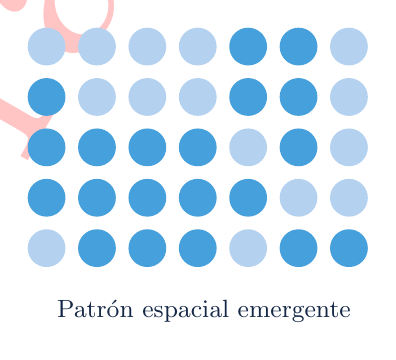
\begin{tikzpicture}[scale=0.8]
					% Patrón de Turing simplificado
					\foreach \i in {0,...,6} {
						\foreach \j in {0,...,4} {
							\pgfmathparse{rand > 0 ? "accentblue" : "lightblue"}
							\fill[\pgfmathresult] (\i*0.8, \j*0.8) circle (0.3cm);
						}
					}
					\node[text=darktext, font=\small] at (2.5,-1) {Patrón espacial emergente};
				\end{tikzpicture}
			\end{column}
		\end{columns}
	\end{frame}
	
	\begin{frame}{El Atlas de Turing: Cartografía de la heterogeneidad metabólica}
		\begin{columns}[T]
			\begin{column}{0.48\textwidth}
				\begin{block}{\color{primaryblue}Patrón 2 (Laberintos)}
					\begin{itemize}
						\item Asociado a estado $P_2$
						\item Frentes de invasión interconectados
						\item Estructuras ramificadas
					\end{itemize}
				\end{block}
				
				\vspace{0.3cm}
				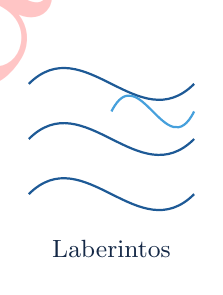
\begin{tikzpicture}[scale=0.7]
					% Patrón tipo laberinto
					\draw[secondaryblue, thick] (0,0) .. controls (1,1) and (2,-1) .. (3,0);
					\draw[secondaryblue, thick] (0,1) .. controls (1,2) and (2,0) .. (3,1);
					\draw[secondaryblue, thick] (0,-1) .. controls (1,0) and (2,-2) .. (3,-1);
					\draw[accentblue, thick] (1.5,0.5) .. controls (2,1.5) and (2.5,-0.5) .. (3,0.5);
					\node[text=darktext, font=\small] at (1.5,-2) {Laberintos};
				\end{tikzpicture}
			\end{column}
			
			\begin{column}{0.48\textwidth}
				\begin{alertblock}{\color{primaryblue}Patrón 3 (Franjas)}
					\begin{itemize}
						\item Asociado a estado $P_3$
						\item Gradientes de señalización direccional
						\item Bandas paralelas
					\end{itemize}
				\end{alertblock}
				
				\vspace{0.3cm}
				
\begin{tikzpicture}[scale=0.7]
					% Patrón tipo franjas
					\foreach \i in {0,...,4} {
						\fill[lightblue] (0, \i*0.6) rectangle (3, \i*0.6+0.3);
					}
					\node[text=darktext, font=\small] at (1.5,-2) {Franjas};
				\end{tikzpicture}
			\end{column}
		\end{columns}
		
		\vspace{0.4cm}
		\begin{block}{\color{primaryblue}Concepto Central}
			Relación directa entre parámetros metabólicos matemáticos y la emergencia espacial de fenotipos tumorales observados clínicamente
		\end{block}
	\end{frame}
	
	\section{Metodología}
	
	\begin{frame}{Cuantificación de la Vulnerabilidad: Índices de Sobol}
		\begin{columns}[T]
			\begin{column}{0.48\textwidth}
				\begin{block}{\color{primaryblue}El Método}
					\begin{itemize}
						\item Perturbación sistemática del modelo dinámico reducido
						\item Identificación \textit{in-silico} de parámetros críticos
						\item Análisis de sensibilidad global
						\item Descomposición de varianza
					\end{itemize}
				\end{block}
				
				\vspace{0.3cm}
				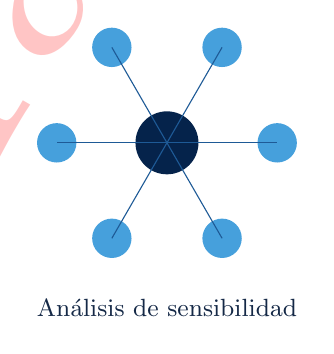
\begin{tikzpicture}[scale=0.7]
					\node[circle, fill=primaryblue, minimum size=0.8cm] at (0,0) {};
					\foreach \i in {1,...,6} {
						\node[circle, fill=accentblue, minimum size=0.5cm] at (360/6*\i:2cm) {};
						\draw[secondaryblue] (0,0) -- (360/6*\i:2cm);
					}
					\node[text=darktext, font=\small] at (0,-3) {Análisis de sensibilidad};
				\end{tikzpicture}
			\end{column}
			
			\begin{column}{0.48\textwidth}
				\begin{alertblock}{\color{primaryblue}El Impacto}
					\begin{itemize}
						\item Parámetros que desestabilizan el tumor
						\item Generación de hipótesis testables
						\item Terapias combinadas dirigidas a la red
						\item Identificación de dianas
					\end{itemize}
				\end{alertblock}
				
				\vspace{0.3cm}
				\begin{center}
					\fbox{\parbox{0.8\linewidth}{\centering \textbf{\color{primaryblue}Atacar la red, no solo la célula}}}
				\end{center}
			\end{column}
		\end{columns}
	\end{frame}
	
	\begin{frame}{Hacia la oncología predictiva: Gemelos Digitales}
		\begin{columns}[T]
			\begin{column}{0.48\textwidth}
				\textbf{\color{primaryblue}Componentes del Sistema:}
				\vspace{0.3cm}
				
				\begin{itemize}
					\item \textbf{Integración multicapa:} Genómica, proteómica y topología clínica
					\item \textbf{Réplicas virtuales dinámicas:} Predicción de trayectorias de resistencia
					\item \textbf{Mejora de algoritmos:} Atención en imagenología clínica
				\end{itemize}
				
				\vspace{0.3cm}
				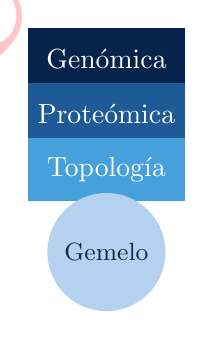
\begin{tikzpicture}[scale=0.7]
					\node[rectangle, fill=primaryblue, minimum width=2cm, minimum height=0.8cm, text=white] at (0,1) {Genómica};
					\node[rectangle, fill=secondaryblue, minimum width=2cm, minimum height=0.8cm, text=white] at (0,0) {Proteómica};
					\node[rectangle, fill=accentblue, minimum width=2cm, minimum height=0.8cm, text=white] at (0,-1) {Topología};
					\node[circle, fill=lightblue, minimum size=1.5cm] at (0,-2.5) {};
					\node[text=darktext, font=\small] at (0,-2.5) {Gemelo};
				\end{tikzpicture}
			\end{column}
			
			\begin{column}{0.48\textwidth}
				\begin{block}{\color{primaryblue}Flujo de Integración}
					\centering
					\vspace{0.2cm}
					\fbox{\parbox{0.85\linewidth}{
							\centering
							Imagenología Clínica\\
							$+$\\
							Red Metabólica\\
							$+$\\
							Datos Genómicos\\
							$\Downarrow$\\
							\textbf{\color{primaryblue}Gemelo Digital Predictivo}
					}}
				\end{block}
				
				\vspace{0.3cm}
				\begin{alertblock}{Aplicación}
					Medicina personalizada y predicción de respuesta terapéutica
				\end{alertblock}
			\end{column}
		\end{columns}
	\end{frame}
	
	\begin{frame}{Hoja de Ruta de la Investigación (24 Meses)}
		\begin{columns}[T]
			\begin{column}{0.48\textwidth}
				\textbf{\color{primaryblue}Cronograma de Actividades}
				\vspace{0.3cm}
				
				\renewcommand{\arraystretch}{1.3}
				\begin{tabular}{lcc}
					\toprule
					\textbf{Actividad} & \textbf{Meses} & \textbf{Estado} \\
					\midrule
					Reconstrucción KEGG & 1-6 & \cellcolor{lightblue} \\
					Análisis Topológico & 1-6 & \cellcolor{lightblue} \\
					Algoritmo Louvain & 7-12 & \cellcolor{lightblue} \\
					Reducción Dinámica & 7-12 & \cellcolor{lightblue} \\
					Estabilidad/Robustez & 13-18 & \cellcolor{lightblue} \\
					Índices de Sobol & 13-18 & \cellcolor{lightblue} \\
					Reacción-Difusión & 19-24 & \cellcolor{lightblue} \\
					Atlas de Turing & 19-24 & \cellcolor{lightblue} \\
					\bottomrule
				\end{tabular}
			\end{column}
			
			\begin{column}{0.48\textwidth}
				\begin{block}{\color{primaryblue}Hitos Principales}
					\begin{itemize}
						\item[\textcolor{primaryblue}{\textbullet}] Mes 6: Red reconstruida
						\item[\textcolor{primaryblue}{\textbullet}] Mes 12: Módulos identificados
						\item[\textcolor{primaryblue}{\textbullet}] Mes 18: Vulnerabilidades cuantificadas
						\item[\textcolor{primaryblue}{\textbullet}] Mes 24: Atlas de patrones
					\end{itemize}
				\end{block}
				
				\vspace{0.3cm}
				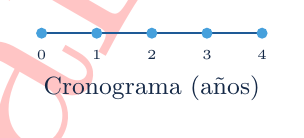
\begin{tikzpicture}[scale=0.7]
					\draw[secondaryblue, thick] (0,0) -- (4,0);
					\foreach \i in {0,1,2,3,4} {
						\fill[accentblue] (\i,0) circle (0.1cm);
						\node[text=darktext, font=\tiny] at (\i,-0.4) {\i};
					}
					\node[text=darktext, font=\small] at (2,-1) {Cronograma (años)};
				\end{tikzpicture}
			\end{column}
		\end{columns}
	\end{frame}
	
	\section{Resultados e Impacto}
	
	\begin{frame}{Conectando Estructura, Dinámica y Espacio}
		\begin{columns}[T]
			\begin{column}{0.32\textwidth}
				\centering
				\begin{block}{\color{primaryblue}\Large Estructura}
					\vspace{0.3cm}
					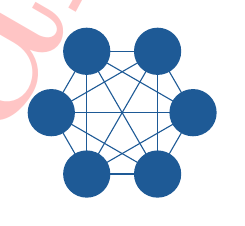
\begin{tikzpicture}[scale=0.6]
						\foreach \i in {1,...,6} {
							\node[circle, fill=secondaryblue, minimum size=0.6cm] at (360/6*\i:1.5cm) {};
						}
						\foreach \i in {1,...,6} {
							\foreach \j in {\i,...,6} {
								\draw[secondaryblue, thin] (360/6*\i:1.5cm) -- (360/6*\j:1.5cm);
							}
						}
					\end{tikzpicture}
					\vspace{0.3cm}
					
					\textbf{Topología}
					\vspace{0.2cm}
					
					Dicta la vulnerabilidad de la red
				\end{block}
			\end{column}
			
			\begin{column}{0.04\textwidth}
				\centering
				\Huge \color{accentblue}$\rightarrow$
			\end{column}
			
			\begin{column}{0.32\textwidth}
				\centering
				\begin{alertblock}{\color{primaryblue}\Large Dinámica}
					\vspace{0.3cm}
					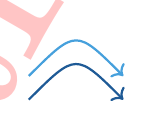
\begin{tikzpicture}[scale=0.6]
						\draw[secondaryblue, thick, ->] (0,0) .. controls (1,1) .. (2,0);
						\draw[accentblue, thick, ->] (0,0.5) .. controls (1,1.5) .. (2,0.5);
					\end{tikzpicture}
					\vspace{0.3cm}
					
					\textbf{Reducción}
					\vspace{0.2cm}
					
					Revela el motor del cáncer
				\end{alertblock}
			\end{column}
			
			\begin{column}{0.04\textwidth}
				\centering
				\Huge \color{accentblue}$\rightarrow$
			\end{column}
			
			\begin{column}{0.28\textwidth}
				\centering
				\begin{block}{\color{primaryblue}\Large Espacio}
					\vspace{0.3cm}
					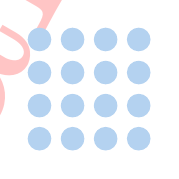
\begin{tikzpicture}[scale=0.6]
						\foreach \i in {0,...,3} {
							\foreach \j in {0,...,3} {
								\fill[lightblue] (\i*0.7, \j*0.7) circle (0.25cm);
							}
						}
					\end{tikzpicture}
					\vspace{0.3cm}
					
					\textbf{Atlas de Turing}
					\vspace{0.2cm}
					
					Mapea el futuro clínico
				\end{block}
			\end{column}
		\end{columns}
		
		\vspace{0.4cm}
		\begin{center}
			\fbox{\parbox{0.7\textwidth}{\centering \textbf{\color{primaryblue}Integración multiescala para oncología de precisión}}}
		\end{center}
	\end{frame}
	
	% Diapositiva final
	\begin{frame}[plain]
		\begin{tikzpicture}[remember picture, overlay]
			% Fondo gradiente
			\shade[top color=primaryblue, bottom color=secondaryblue] 
			(current page.south west) rectangle (current page.north east);
			
			% Agradecimiento
			\node[anchor=center, align=center, text=textwhite, font=\bfseries\Large] 
			at (current page.center) 
			{¡Gracias por su atención!};
			
			\node[anchor=center, align=center, text=lightblue, font=\normalsize] 
			at ([yshift=-1.5cm]current page.center) 
			{Preguntas y comentarios};
			
			% Información de contacto
			\node[anchor=south, align=center, text=textwhite, font=\small] 
			at ([yshift=3cm]current page.south) 
			{Alejandro Guerra González\\
				Posgrado de Ciencias en Ingeniería Química\\
				Facultad de Ciencias Químicas, UASLP\\
				\vspace{0.3cm}
				Asesor: Dr. Erik César Herrera Hernández};
		\end{tikzpicture}
	\end{frame}
	
\end{document}